\chapter{Revisão Teórica} \label{revisão}
% [Futuramente, pode ser necessário expandir essa seção]

Esta seção visa oferecer os conceitos necessários para o completo entendimento desse trabalho. Inicialmente, serão apresentados os conceitos relacionados a classificação de satélites, o padrão CubeSat, alguns conceitos de eletrônica e, por fim, um histórico das missões anteriores com enfoque nos sistemas de potência utilizados.

\section{Nanossatélites}\label{nanosats_revision}
Normalmente, a classificação mais utilizada para satélites é com relação a sua massa. Na figura abaixo, podemos ver as categorias utilizadas nessa classificação e alguns exemplos de artefatos já lançados. Observe que os nanossatélites se encontram na faixa de 1 até 10 kg.

\noindent
\begin{minipage}{\linewidth}
\makebox[\linewidth]{
    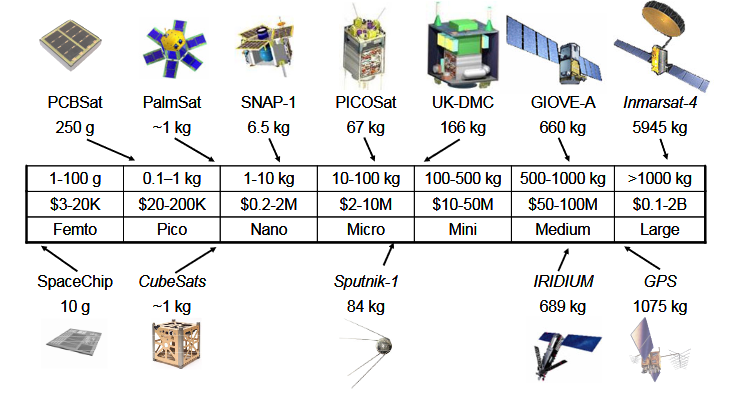
\includegraphics[keepaspectratio=true, scale=0.5]{imagens/Satellite-mass-classification.png}}
\label{mass_classification_fig}
\captionof{figure}{Classificação de satélites, com alguns exemplos}
\end{minipage}

 Os principais responsáveis por essa redução de massa são a miniaturização dos circuitos integrados e as padronizações das estruturas de lançamento, como no padrão \textit{Cubesat}. Os nanossatélites são amplamente utilizados nas atividades de ensino, pois permitem um ciclo completo de uma missão espacial mantendo um custo baixo, principalmente devido ao uso de peças comerciais.\cite{barnhart_ref}

\section{\textit{Cubesat}}\label{cubesat_revision}

O padrão \textit{Cubesat} foi um dos grandes responsáveis pela popularização da categoria de nanossatélites, como podemos ver no gráfico abaixo, que mostra o número de lançamentos desse tipo por ano.\cite{cubesats_cgee}.

\noindent
\begin{minipage}{\linewidth}
\makebox[\linewidth]{
    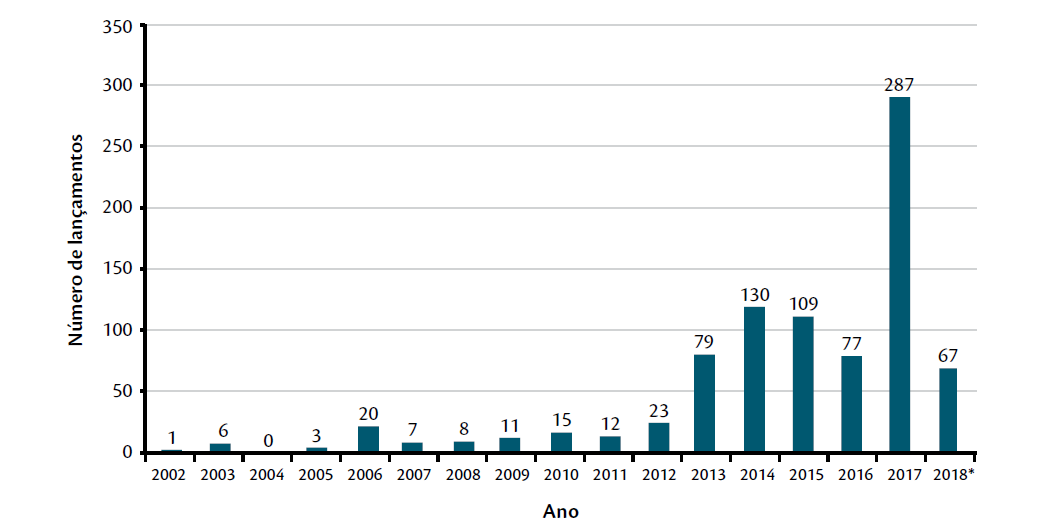
\includegraphics[keepaspectratio=true, scale=0.5]{imagens/cubesat-launches-count.png}}
\captionof{figure}{Distribuição do número de \textit{Cubesats} pelo ano de lançamento}
\label{cubesat_launches_fig}
\end{minipage}

O modelo \textit{Cubesat} foi proposto em 1999 por Jordi Puig-Suari, da \textit{California Polytechnic State University}, e Bob Twiggs, da \textit{Stanford University}. O objetivo era um modelo de satélite de pequeno porte que segue um padrão mais simples, o intuito deles era fornecer aos alunos de ambas universidades a oportunidade de  participar de um projeto espacial completo, incluindo todas as fases, desde a construção, testes e operação do artefato, que manteria características similares aos satélites maiores. 

O termo é um acrônimo entre as palavras \textit{cube} (em inglês, cubo) acrescida das três primeiras letras da palavra satélite.

Normalmente, as missões com \textit{Cubesats} tem um risco técnico mais elevado, em parte devido ao uso de componentes não \textit{"space qualified"}, porém oferecem em troca uma implementação mais rápida, aplicações mais inovadoras, custos menores ou um conjunto desses elementos.

As principais características dos \textit{Cubesats} são as seguintes:
\begin{itemize}
    \item compostos por unidades cúbicas padronizadas (1U) de tamanho 10x10x10 cm, conforme mostrado na figura \ref{cubesat_configs_fig};
    \item uso de sistemas padronizados de ejeção em órbita, denominados, P-POD (do inglês, \textit{Poly Picosatellite Orbital Deployer}) ou SSPL (do inglês, \textit{Space Shuttle Picosatellite Launcher}). Esses sistemas são capazes de liberar diversos satélites pela mesma interface;
    \item componentes COTS nos sistemas de bordo.
\end{itemize}

\noindent
\begin{minipage}{\linewidth}
\makebox[\linewidth]{
    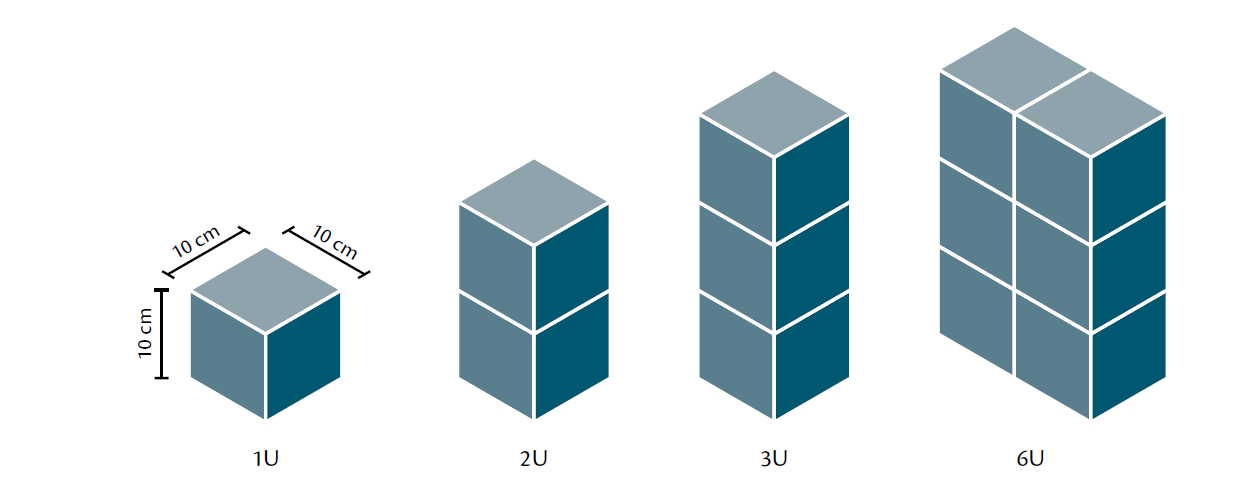
\includegraphics[keepaspectratio=true, scale=0.5]{imagens/cubesats-configs.png}}
\captionof{figure}{Algumas configurações de \textit{Cubesats}}
\label{cubesat_configs_fig}
\end{minipage}

O padrão é descrito em um documento de domínio público\cite{cubesat_specs_rev13}, onde especifica-se que uma unidade \textit{Cubesat} ou 1U, tem um volume de 1 litro e carga útil de até 1,3 kg, podendo combinar várias unidades dessas para compor satélites maiores (2U, 3U, 6U ou 12U, por exemplo).

Quanto aos requisitos elétricos, o padrão apresenta dois requisitos extremamente importantes que são o \textit{Deployment Switch} e o pino \textit{Remove Before Flight} (RBF).
\begin{enumerate}
    \item O \textit{Deployment Switch} é uma chave que deve desconectar eletricamente todos os subsistemas, sem exceções, do sistema de potência.
    \item Essa chave deve atuar durante todo o tempo que o CubeSat estiver acoplado no P-POD, e esse sinal é recebido dos trilhos do P-POD, conforme figura X.
    \item Por sua vez, o RBF, é um pino que deve cortar toda a alimentação do satélite uma vez que estiver inserido. Ele será removido após o encaixe na base de lançamento P-POD e não deve avançar mais do que 6.5 mm além dos trilhos.
\end{enumerate}

\noindent
\begin{minipage}{\linewidth}
\makebox[\linewidth]{
    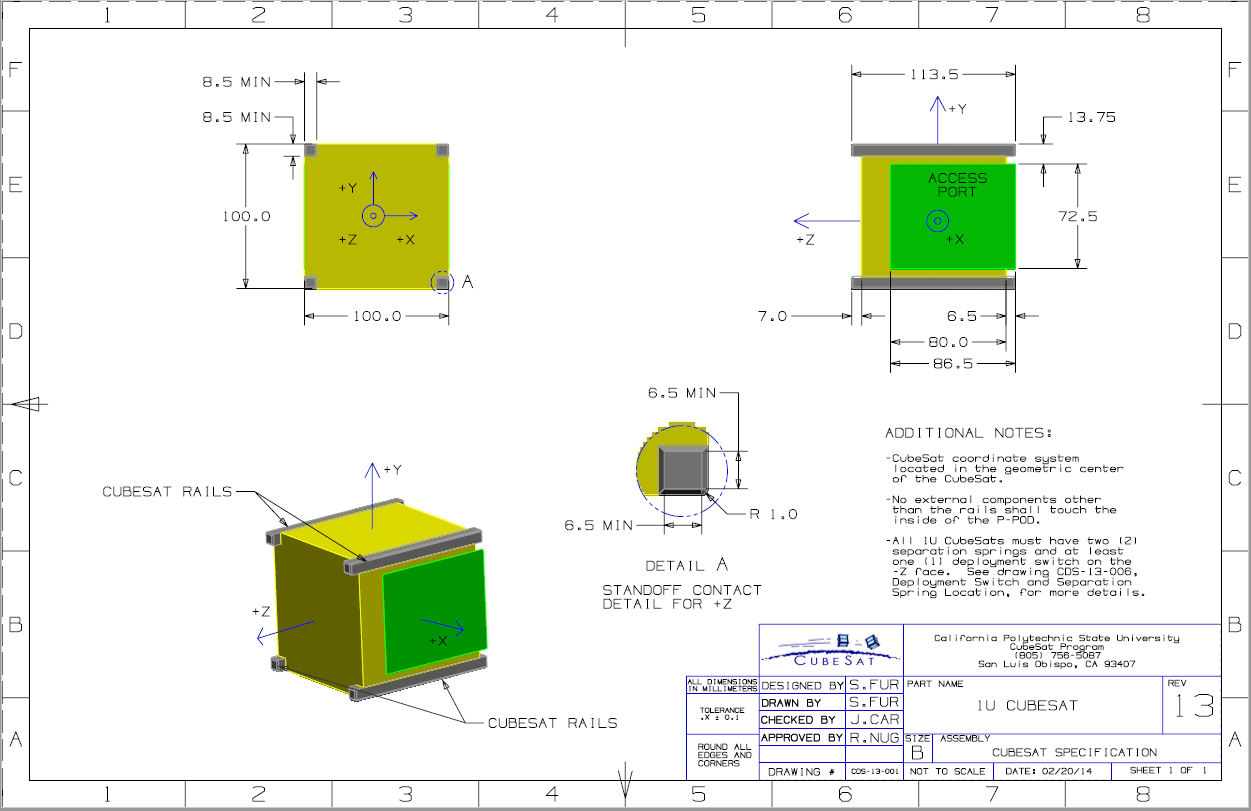
\includegraphics[keepaspectratio=true, scale=0.5]{imagens/Cubesat-diagram.png}}
\captionof{figure}{Especificações de dimensionamento para um \textit{Cubesat} 1U}
\label{cubesat1U_dimensions_fig}
\end{minipage}

Por esses e outros aspectos, os \textit{Cubesats} trouxeram um aspecto inovador capaz de mudar o paradigma do setor espacial, adequando-o à nova tendência de emprego de pequenos satélites para atender a diferentes tipos de demandas.

%\section{Printed Circuit Board (PCB)}\label{pcb_revision}
%\textit{Printed Circuit Board}, em português: placa de circuito impresso, é uma técnica amplamente utilizada na eletrônica que consiste em construir uma placa de um material isolante que apresenta em sua superfícies trilhas condutoras que representam o circuito em que serão soldados os dispositivos eletrônicos.

%Para a maioria dos circuitos, ter apenas uma superficie condutora é insuficiente dado que algum momento durante o design será impossível evitar o cruzamento entre trilhas, portanto, a maioria das PCBs são multicamadas, ou seja, possuem múltiplas camadas de trilhas condutoras isoladas.

%Essa forma de construir circuitos representou grande avanço na eletrônica, pois esse arranjo permite maior resistência a interferências, melhor fixação dos componentes e otimização no uso do espaço, possibilitando equipamentos menores.

%O processo moderno de design de uma PCB é facilitado pelo uso de software de \textit{layout} dedicado que ao final do processo nos fornece os arquivos .gerber que serão usados para a fabricação, nesses arquivos não são colocadas informação sobre os componentes, há apenas as informações que o fabricante da PCB necessita, a exemplo das \textit{layers}, furações, entre outros.

\section{Paineis Solares}
Os painéis solares, ou PV\footnote{Photovoltaics - conforme literatura em inglês sobre o assunto}, são dispositivos que utilizam o efeito fotovoltaico para produzir energia elétrica. Nas células solares, a diferença de potencial surge quando um elétron recebe energia suficiente para passar da camada de valência para a camada de condução do material semicondutor.

Diferente dos metais, os semicondutores possuem a camada de valência completamente cheia e a camada de condução completamente vazia, e o salto "\textit{gap}" entre as duas camadas é de 1 eV (elétron-volt). Caso o fóton incidente na placa forneça mais energia do que o necessário para o elétron atravessar o salto, o excesso se transforma em calor, em um efeito conhecido por termalização.

\subsection*{Curva I-V}
A curva I-V\footnote{Curva Corrente x Tensão} é uma das caracteristicas mais importantes quando projeta-se algo com painel solar, pois é necessário conhecer e realizar a previsão de parâmetros importantes como a irradiação solar, temperatura e carga que será atendida. A maioria dos métodos presentes na literatura utiliza a curva I-V para o cálculo desses parâmetros ou então outros métodos de natureza empírica, a seguir vamos usar essa técnica\cite{pv_datasheet} para montar um modelo para as simulações.

\subsection*{Modelo para simulação}
A curva I-V geral de um painel solar é baseada no modelo exponencial \cite{pv_datasheet}:
\begin{equation}
    i = I_{ph} - I_{o}(e^{\frac{v + iR_{s}}{n_{s}V_{t}}}-1) - \frac{v + iR_{s}}{R_{sh}}
\end{equation}
Na equação acima, $V_{t}$ é a tensão térmica da junção P-N.
\begin{equation}
    V_{t} = \frac{AkT_{stc}}{q}
\end{equation}
Com esses parâmetros, forma-se o seguinte circuito equivalente para uma célula solar:
\noindent
\begin{minipage}{\linewidth}
\makebox[\linewidth]{
    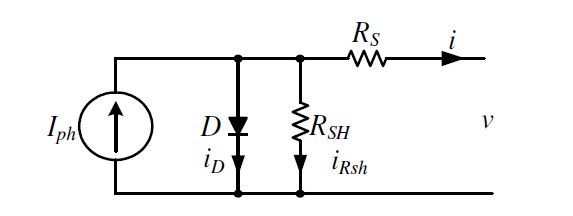
\includegraphics[keepaspectratio=true, scale=0.5]{imagens/PV_eq_circuit.PNG}}
\captionof{figure}{Circuito equivalente para uma célula fotovoltaica, usando o modelo exponencial}
\label{PV_equivalent_circuit_fig}
\end{minipage}
Onde os parâmetros do modelo são,
\begin{itemize}
    \item $I_{ph}$ - Corrente gerada pela célula
    \item $I_{o}$ - Corrente de saturação
    \item $R_{s}$ - Resistência em série da célula
    \item $R_{sh}$ - Resistência em paralelo da célula (shunt)
    \item $A$ - Fator de qualidade do diodo
\end{itemize}
Além desses parâmetros, $k$ é a constante de Boltzmann, $q$ é a carga do elétron, $n_{s}$ é o número de células conectadas em série, e $T_{stc}$ ($K$) é a temperatura na STC\footnote{STC, sigla para \textit{Standard Test Conditions}, condições de teste para aferir as medidas de caracterização de um painel solar.}.

\subsection*{Ponto de máxima potência}

\textbf{Pendente}

\section{Conversores DC-DC}\label{converters_revision}
Conversores DC-DC são dispositivos eletrônicos capazes de converter uma tensão de entrada em um tensão diferente e, normalmente, provê uma saída regulada. Os conversores to tipo chaveados estão cada vez mais comuns devido a alta eficiência e por permitir uma flexibilidade de projeto, ou seja, da mesma tensão de saída é possível gerar multiplas tensões de saída de projetos diferentes. As próximas subseções detalharão brevemente os princípios de funcionamento de quatro das topologias mais comumente utilizadas.

%TODO: Falar que você precisa apenas do circuito abaixador de tensão e que irá comparar os circuitos BUCK e o SEPIC. Não é de interesse deste projeto avaliar conversores elevadores de tensão, como Boost, buck-boost.

Antes de continuarmos para as topologias, inicialmente, vamos entender o significado de ser chaveado. Em um circuito chaveado, existirá um transistor que atuará como chave, ou seja, alterar entre os estados completamente ligado e completamente desligado. Para um transistor do tipo BJT isso significa transicionar entre os estados de corte e saturação, no transistor do tipo MOSFET, entre os estados de corte e triodo. 

%TODO: Considerar mesclar essa seção com a seção do conversor Buck.
\subsection{Pulse Width Modulation (PWM)}
Todos os conversores abordados abaixo, usam uma forma de regulação da tensão de saída conhecido como modulação por largura de pulso, ou \textit{PWM - Pulse Width Modulation}. Simplificadamente, o loop de feedback ajusta a tensão de saída alterando o tempo em que a chave, ou o elemento comutador, do conversor ficará ligada.

\noindent
\begin{minipage}{\linewidth}
\makebox[\linewidth]{
    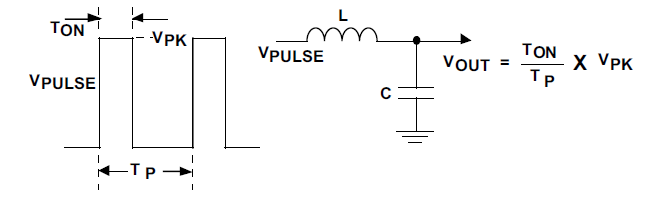
\includegraphics[keepaspectratio=true, scale=0.5]{imagens/PWM_sample.png}}
\captionof{figure}{Exemplo de uma saída PWM}
\label{PWM_sample_fig}
\end{minipage}

A saída na forma de onda quadrada é filtrada e fornece uma tensão de saída DC igual ao valor da tensão de pico $V_{pk}$ multiplicada pelo \textit{Duty Cycle}, que é a razão entre o período ligado e o período local. Esta relação explica como a tensão de saída conversor pode ser diretamente controlada apenas alterando o Duty Cycle.  

\subsection{Topologia Buck}
A topologia de conversor chaveado mais utilizada é a \textit{Buck}, utilizada para converter uma tensão DC para uma tensão DC menor e de mesma polaridade. O conversor \textit{buck} utiliza um transistor para chavear a tensão de entrada para o indutor, conforme observado no circuito abaixo:

\textbf{ Inserir circuitos Buck }

Para avaliar o funcionamento de circuito, vamos considerar dois momentos, quando a chave está fechada e quando a chave está aberta.



%\subsection{Topologia Boost}
%A topologia \textit{Boost}, como o próprio nome sugere, produz uma tensão DC de saída maior que a tensão de entrada e de mesma polaridade. 

%\textbf{ Inserir circuitos Boost }

%Novamente, vamos avaliar os períodos com a chave fechada e aberta.



%\subsection{Topologia Buck-Boost}
%A topologia \textit{Buck-Boost} é uma derivação das duas primeiras, de tal forma que é possível, dada uma tensão de entrada, produzir uma tensão de saída maior do que ela e de mesma polaridade, ou uma tensão menor, porém com inversão de polaridade.

%\textbf{ Inserir circuitos Buck-Boost }

\subsection{Topologia SEPIC}
O nome SEPIC (\textit{Single-Ended Primary Inductance Converter}), ou, em tradução livre, Conversor com Indutância Simples no Primário é um conversor capaz de converter uma tensão DC de entrada para um tensão DC maior ou menor, porém sem que ocorra inversão de polaridade. Essa característica traz uma versatilidade muito boa para essa topologia de conversor, uma vez que a inversão de polaridade costuma ser indesejada em muito projetos. 

\textbf{ Inserir circuitos Sepic }


\section{MPPT - Maximum Peak Point Tracking}\label{mppt_revision}
Ao caracterizar o painel solar da GOMSpace, os resultados da simulação usando o modelo exponencial mostraram que a configuração em que o painel é conectado diretamente a bateria, sem o auxílio de um controlador de carga, causa uma situação de baixa eficiência, pois dificilmente a célula estara funcionando no seu ponto ótimo nessas circunstâncias.

A técnica MPPT, Rastreamento do Ponto de Máxima Potência, em tradução livre, é usada para extrair a máxima potência de um painel solar e transferi-la para a carga. Para atingir esse objetivo, um conversor DC/DC é utilizado com interface entre a carga e o painel solar, de tal forma que ao alterar o \textit{duty cycle} a impedância vista pela fonte varia para combinar com o ponto de máxima potência e assim transferir a máxima potência para a carga. A seguir, faremos uma comparação entre dois algoritmos bastante populares para implementação da técnica MPPT \cite{mppt_comparison}.

\subsection{Algoritmo: Pertuba e Observa}
O Pertuba e Observa, também conhecido como P\&O, é um algoritmo iterativo que analisa a potência do circuito em tempos discretos e com essas informações toma uma decisão de qual ajuste deve ser feito no circuito. 

\noindent
\begin{minipage}{\linewidth}
\makebox[\linewidth]{
    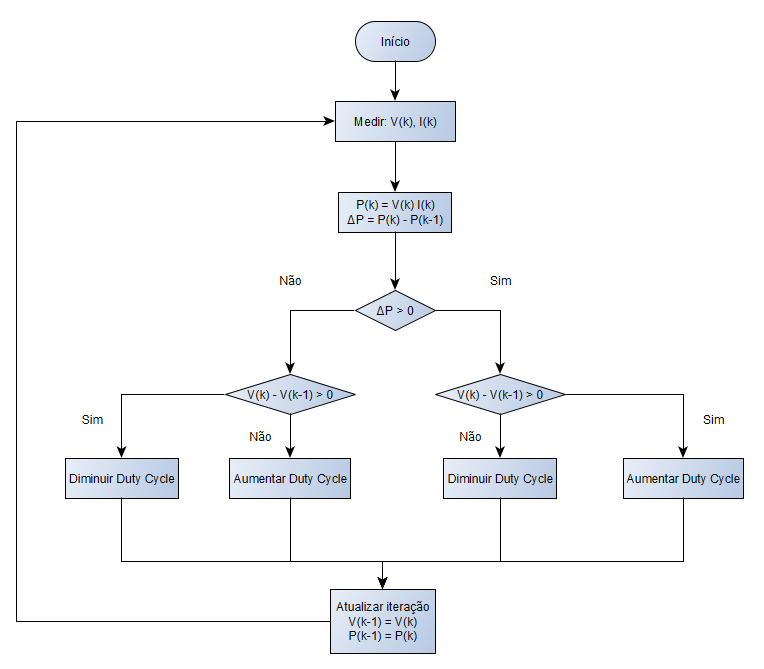
\includegraphics[keepaspectratio=true, scale=0.5]{imagens/P&O_flux.png}}
\captionof{figure}{Fluxograma para o algoritmo Perturba e Observa}
\label{PO_flux_fig}
\end{minipage}

No inicio do ciclo, o primeiro passo é aferir a tensão e corrente na carga. Com esses dados, calcula-se o $\Delta$P (variação da potência) entre a iteração atual e a anterior, em seguida, avalia-se se a tensão é maior ou menor do que a observada na iteração anterior. Com todos esses dados adquiridos, surgem quatro ramos de decisão:
\begin{enumerate}
    \item A potência aumentou e a tensão aumentou: aumentar o \textit{Duty Cycle} no conversor 
    \item A potência aumentou e a tensão diminuiu: diminuir o \textit{Duty Cycle} no conversor
    \item A potência diminuiu e a tensão aumentou: diminuir o \textit{Duty Cycle} no conversor
    \item A potência diminuiu e a tensão diminuiu: aumentar o \textit{Duty Cycle} no conversor
\end{enumerate}

Após fazer as correções no conversor, os valores dessa iteração são salvos para serem usado posteriormente como comparação com a iteração seguinte. O algoritmo P e O é amplamente utilizado devido a simplicidade de implementação e boa eficiência. Um ponto desfavorável desse algoritmo é que ele não consegue atingir uma estabilidade quando próximo do ponto de máxima potência, uma vez que ele sempre estará avaliando e tentando ajustar o circuito.

\subsection{Algoritmo: Condutância Incremental}

O algoritmo da Condutância Incremental (CI) corrige um dos problemas do Pertuba e Observa que é a estabilidade quando se atinge o ponto de máxima potência, o algoritmo é capaz de determinar que esse ponto foi atingindo e não mais alterar a configuração de operação. Além disso, ele é capaz de reagir com melhor precisão as mudanças abruptas de irradiação, a desvantagem em relação ao algoritmo P\&O é com a sua maior complexidade de implementação. Abaixo, segue o fluxograma e a explicação do algoritmo CI.

\noindent
\begin{minipage}{\linewidth}
\makebox[\linewidth]{
    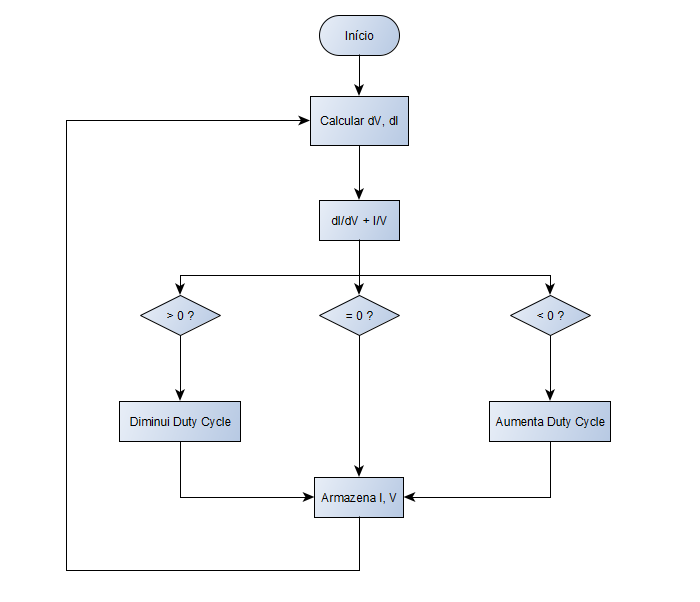
\includegraphics[keepaspectratio=true, scale=0.5]{imagens/CI_flux.png}}
\captionof{figure}{Fluxograma para o algoritmo Condutância Incremental}
\label{CI_flux_fig}
\end{minipage}

Se a condição de equilibrio não for encontrada, a direção em que o ponto de operação MPPT deve ser perturbado, realizando a alteração no $\frac{dI}{dV}$ e $\frac{-I}{V}$. Essa relação é derivada do fato de que $\frac{dP}{dV}$ é negativo quando o MPPT está à direita do ponto de máxima potência e positivo quando está à esquerda.

%\section{Microcontrolador/Microprocessador}\label{mcu_revision}
%A principal diferenciação entre microcontroladores e microprocessadores está na quantidade de componentes que estão embarcados em um e outro. O microcontrolador (MCU) é um computador completo inteiro em um único circuito integrado, ou seja, contém memórias, timers, portas de comunicação serial, entre outros periféricos. Já o microprocessor contém essencialmente as unidades de controle e cálculo, necessitando de periféricos externos para formar um sistema minímo de um computador.

%Os MCUs atualmente encontram uma enorme gama de aplicações na eletrônica moderna, desde máquinas industriais, sistemas embarcados a brinquedos e eletrodomésticos. São exemplos de microcontroladores: Texas Instruments MSP430, PIC, Atmel AVR, ARM Cortex-M, entre outros.

%\noindent
%\begin{minipage}{\linewidth}
%\makebox[\linewidth]{
%    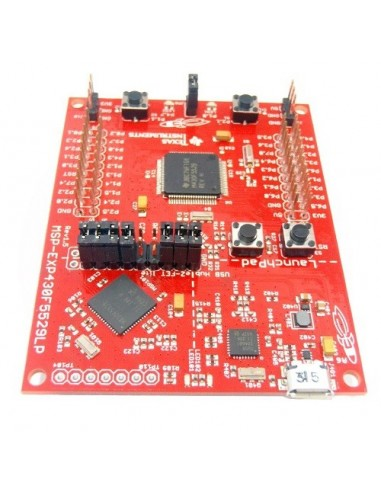
\includegraphics[keepaspectratio=true, scale=0.5]{imagens/msp-exp430f5529lp.jpg}}
%\captionof{figure}{Placa de desenvolvimento com um microcontrolador MSP430F5529}
%\label{uC_MSP430_sample_fig}
%\end{minipage}

%Para a nossa missão, existirão vários MCUs espalhados em diversos subsistemas do nanossatélites, desempenhando funções distintas. Abaixo seguem %alguns critérios importantes na escolha do MCU mais adequado:

% \begin{enumerate}
%     \item Baixo consumo: a disponibilidade de energia em órbia dependerá da área de cobertura e eficiência dos painéis solares e essa potência também será dividida com os outros subsistemas, logo, o nosso MCU tem que consumir pouco quando em funcionamento;
%     \item Conversores AD: O OBC necessitará ler dados de muitos sensores, exemplo: temperatura e luminosidade;
%     \item Portas I/O: As portas GPIO (do inglês \textit{General-Purpose Input/Output}) são essenciais para comunicação com os outros subsistemas;
%     \item Interfaces Seriais: Ter pinos dedicados aos protocolos de comunicação serial (UART, I2C, SPI) ajudam no desenvolvimento do OBC;
%     \item PWM: Para o controle de motores, consequentemente há necessidade de pinos que produzam PWM;
%     \item Frequência de Operação: Deseja-se usar um microcontrolador com uma frequência de \textit{clock} elevada para ter uma melhor performance;
%     \item Faixa de temperatura: O microcontrolador deve resistir a qualquer temperatura encontrada na órbita LEO.
% \end{enumerate}

% Para cada subsistema, a escolha do microcontrolador priorizará certos itens em detrimento de outros, por exemplo, no contexto do EPS, os conversores AD serão o centro das discussões e comparações entre os modelos, já para o contexto do OBC, consumo de energia e capacidade de processamento serão items mais relevantes.

% Mais adiante, no capítulo de desenvolvimento (\ref{desenvolvimento}) abordaremos a nossa escolha de microcontrolador e como esses e outros critérios foram avaliados.


%\subsection{Ambiente espacial}
% Um problema a ser considerado no desenvolvimento, especialmente das placas eletrônicas, é o efeito do ambiente espacial nos subsistemas. Os problemas causados podem variar desde mal funcionamento até danos físicos, normalmente essas considerações são feitas para missões de longa duração realizadas em \textit{LEO} (do inglês \textit{Low Space Orbit}) e \textit{Deep Space} \cite{nasa_state_of_art}.

% A quantidade de radiação que incide nos satélites depende da altitude e do tipo da órbita. A maioria dos \textit{Cubesats} são colocados em órbitas LEO (entre 100 e 1000 km de altitude), recebendo uma dose de radiação de  aproximadamente 0,1 krad/ano.

% A resistência a radiação é um dos grandes desafios das missões \textit{Cubesat}, pois os componentes COTS não tem nenhuma preocupação com radiação durante o processo de design, logo, os clientes desses componentes devem blindar todas as partes eletrônicas, realizar todos os testes de exposição e assumir os possíveis riscos de falhas.
